% Model-derived energy geometry and input authority at single-column width.
\begin{figure}[t]
\centering
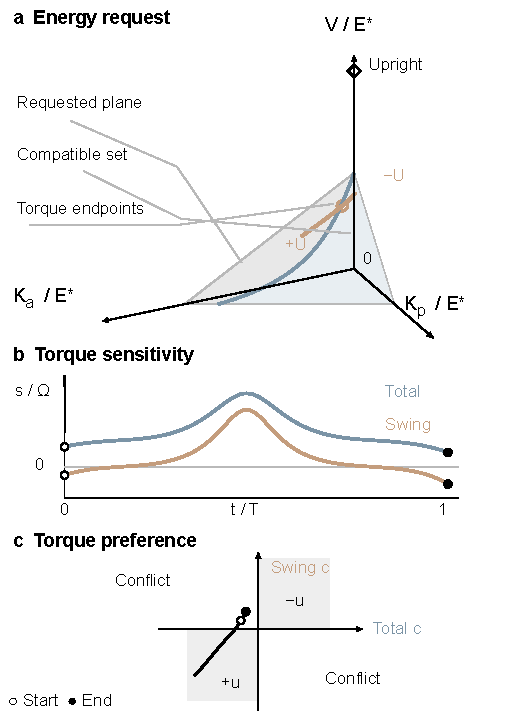
\includegraphics[width=\columnwidth]{figures/energy-control/figure-3-energy-control.pdf}
\caption{Energy requests and state-dependent input directions.
(a) The requested-work plane satisfies $K_a+K_p+V=E+w$, where $E$ is the initial total energy and $w$ is the teacher's requested work. Its blue subset contains mechanically compatible energy distributions, obtained by minimizing pendulum-body kinetic energy over the hinge speed at each arm energy and potential. The orange curve contains endpoints under constant torques in $[-U,U]$ over one fixed duration; the open circle marks work matching. Neither set is a complete bounded-input reachable set. Axes use upright-rest energy $\Estar$, denoted $E^*$ in the artwork; the diamond is $(0,0,\Estar)$.
(b) Blue total-energy and orange relative-swing sensitivities from Eq.~\eqref{eq:energy-authority}, divided by the model's downward small-motion frequency $\Omega>0$, along a constructed zero-input segment. Time is divided by $T=2\pi/\Omega$.
(c) The same segment in $(c_E,c_h)/(\Estar\Omega)$ coordinates. Gray quadrants admit the indicated common torque sign for reducing both input contributions; the other quadrants indicate conflict, and zero axes indicate zero corresponding direct authority. Open and filled markers identify segment start and end. Natural transfer remains in the complete swing-energy rate; these diagnostics do not certify coast duration, arm admissibility, or closed-loop performance.}
\label{fig:energy-control}
\end{figure}
